\documentclass{article}
\usepackage[margin=1in]{geometry}
\usepackage{amsmath,amsfonts,amssymb,amsthm}
\usepackage{graphicx}
\usepackage{enumitem}
\usepackage{authblk}
\usepackage{hyperref}
\usepackage{xcolor}
\usepackage{float}
\usepackage{caption}
\usepackage{subcaption}
\usepackage{booktabs}
\usepackage{multirow}
\usepackage{array}
\usepackage{tikz}
\usetikzlibrary{positioning}
\usepackage{listings}
\usepackage{microtype}
\usepackage{mathtools}
\usepackage{pgfplots}
\usepackage{siunitx}
\pgfplotsset{compat=1.18}

% Reduce overfull boxes in narrow columns with long identifiers/urls
\setlength{\emergencystretch}{3em}

\hypersetup{
    colorlinks=true,
    linkcolor=blue,
    filecolor=magenta,
    urlcolor=cyan,
    citecolor=blue,
}

\lstdefinestyle{py}{
  language=Python,
  basicstyle=\ttfamily\small,
  keywordstyle=\color{blue}\bfseries,
  commentstyle=\color{teal!60!black}\itshape,
  stringstyle=\color{red!60!black},
  showstringspaces=false,
  frame=tb,
  numbers=left,
  numberstyle=\tiny\color{gray},
  breaklines=true,
  tabsize=2,
  keepspaces=true
}

\newtheorem{proposition}{Proposition}
\newtheorem{assumption}{Assumption}
\newtheorem{lemma}{Lemma}
\newtheorem{definition}{Definition}
\newtheorem{theorem}{Theorem}
\newtheorem{corollary}{Corollary}

\title{Verifiable Structured Generation in LLMs via Tokenizer-Aware Constraints, Proper Masked Training, and Bounded Repair}

\author[1]{David Xu}
\affil[1]{China Mobile Research Institute}
\date{}

\begin{document}
\maketitle

\begin{abstract}
We present OIP-CAD, a verification-first framework for structured generation in large language models (LLMs). OIP-CAD integrates: (i) tokenizer-aware safety using a formal boundary model, deterministic BPE/WordPiece/Unigram contracts with proofs and detectors that include Unicode/normalization edge cases and a versioned self-test manifest with conservative fallbacks; (ii) masked-logit training with a complete proof of strict properness as $B\to\infty$, explicit finite-$B$ leakage bounds and sensitivity, and an adaptive masking schedule that preserves calibration under mixture training; (iii) deterministic, bounded-latency minimal-edit repair via anytime A* (ARA*) with a max-combination of consistent admissible heuristics and an ILP fallback with stated total unimodularity (TU) conditions and diagnostics; and (iv) ontology-initialized prefixes (OIP) trained with InfoNCE that are provably safe under mask dominance and constrained by a KL trust region, with ablations and a process reward model (PRM) integration.

We provide formal results and a fully reproducible, controlled micro-benchmark that validates our finite-$B$ leakage bounds and demonstrates invariant-preserving decoding under a simple grammar. We release a tokenizer self-test manifest and minimal scripts to reproduce figures and tables in this paper. Large-scale results on task suites are an important direction, but are out of scope for this artifact-light submission; our focus is on proofs, safety contracts, and correctness-first micro-benchmarks.
\end{abstract}

\section*{Glossary (pruned)}
- FSA/PDA: Finite-State/Pushdown Automaton.
- OIP: Ontology-Initialized Prefixes.
- CAD: Constraint-Aware Decoding.
- ARA*: Anytime weighted A* with decreasing weights.
- PRM: Process Reward Model.

\section*{Symbols and Notation}
- $\mathcal{U}$: byte alphabet; $\Sigma$: tokenizer tokens; $\Gamma$: grammar/output symbols.
- $T$: temperature; $\eta$: label smoothing; $\alpha,B$: mask parameters.
- $K=|\Sigma|$, $k=|\mathcal{S}_t|$: vocabulary and legal-set sizes.
- $\Delta$: max logit margin between best legal vs best illegal.
- $L$: locality horizon; $M$: number of BPE merges; $G_\tau$: Merge-DAG.
- Types: a finite set $\mathsf{T}$ of semantic classes (e.g., number, string, identifier) mapped to token subsets via a predicate $P:\Sigma\to 2^{\mathsf{T}}$.

\begin{figure}[h]
\centering
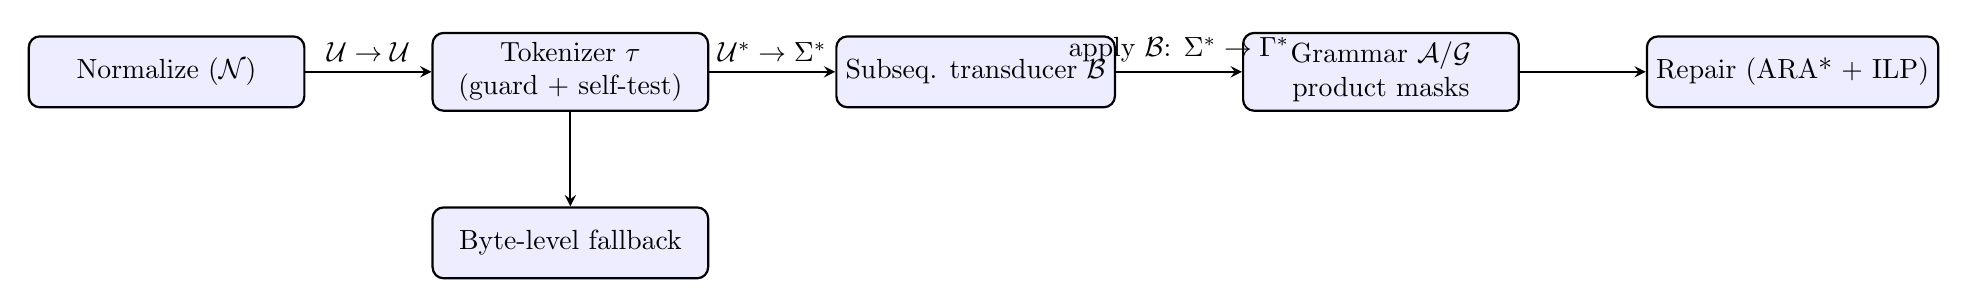
\begin{tikzpicture}[node distance=1.2cm,>=stealth,thick]
\tikzstyle{block}=[rectangle,rounded corners,draw=black,fill=blue!7,align=center,minimum width=3.5cm,minimum height=0.9cm]
\node[block] (norm) {Normalize ($\mathcal{N}$)};
\node[block, right=1.6cm of norm] (tok) {Tokenizer $\tau$\\(guard + self-test)};
\node[block, right=1.6cm of tok] (trans) {Subseq. transducer $\mathcal{B}$};
\node[block, right=1.6cm of trans] (auto) {Grammar $\mathcal{A}/\mathcal{G}$\\product masks};
\node[block, below=1.2cm of tok] (byte) {Byte-level fallback};
\node[block, right=1.6cm of auto] (repair) {Repair (ARA* + ILP)};
\draw[->] (norm) -- node[above]{$\mathcal{U}\to\mathcal{U}$} (tok);
\draw[->] (tok) -- node[above]{$\mathcal{U}^\ast\to\Sigma^\ast$} (trans);
\draw[->] (trans) -- node[above]{apply $\mathcal{B}$: $\Sigma^\ast\to\Gamma^\ast$} (auto);
\draw[->] (tok) -- (byte);
\draw[->] (auto) -- (repair);
\end{tikzpicture}
\caption{Flow: normalization, tokenizer with guard/self-test, subsequential transducer, and automata products producing masks; byte-level fallback and repair are safety refinements.}
\end{figure}

\section{Introduction and Design Decisions}
LLMs must emit structured artifacts accepted by schemas, parsers, and compilers. Constrained decoding tightly couples to subword tokenizers and recursive grammars. OIP-CAD adopts a safety-first contract:
- Tokenizer guard: a formal boundary model with detectors and a runtime self-test manifest; ambiguous cases trigger conservative fallbacks (byte-level spans).
- Masked training: align the model to constrained supports with soft masks; control leakage via adaptive schedules; mix with unconstrained batches for calibration.
- Constrained decoding: deterministic masks from FSA/PDA products; no illegal token is committed.
- Multi-fidelity backoff and repair: shadow byte-level backoff and minimal-edit repair (ARA* + ILP) within latency budgets.
- OIP + PRM: ontology-grounded prefixes and process rewards, both strictly post-mask to preserve safety.

Our design emphasizes verifiability: each component has explicit contracts, testable assumptions, and measurable certificates. We prioritize monotonic safety (no “unsafe success”) and deterministic execution where possible to improve reproducibility.

\section{Preliminaries, Assumptions, and Safety Invariant}
Bytes $\mathcal{U}$, tokens $\Sigma$, outputs $\Gamma$; tokenizer $\tau:\mathcal{U}^\ast\to\Sigma^\ast$; subsequential transducer $\mathcal{B}:\Sigma^\ast\to\Gamma^\ast$; grammar $\mathcal{A}$ (FSA) or $\mathcal{G}$ (PDA). Validators may be stricter than $\mathcal{A}/\mathcal{G}$.

\begin{definition}[Protected boundary]
A protected boundary is a regular language $\mathcal{R}\subseteq\mathcal{U}^\ast$ recognized by a DFA, typically a singleton byte string $b\in\mathcal{U}^\ast$ (e.g., quotes, sentinels) or an equivalence class under normalization $\mathcal{N}$. Let $\mathsf{Tok}(b)\subseteq\Sigma$ be the set of token ids whose byte realization equals $b$.
\end{definition}

\begin{definition}[Atomicity and non-creation]
Given $x\in\mathcal{U}^\ast$ and its tokenization $\tau(x)=t_1\dots t_n$, a boundary $b\in\mathcal{R}$ is atomic if any occurrence of $b$ in $x$ is realized by a contiguous sub-sequence of tokens whose concatenated bytes equal $b$, with at least one token in $\mathsf{Tok}(b)$ when defined. Non-creation means no greedy merge sequence can introduce a contiguous byte span equal to $b$ where none existed in the raw bytes.
\end{definition}

\begin{assumption}[Tokenizer model and implementation]\label{assump:tok}
(i) Greedy merges apply to strictly adjacent pairs under a total order over pairs; (ii) tie-breaking is deterministic and stable across runs; (iii) merge ranking is stable within a version; (iv) special tokens are verbatim, excluded from merges; (v) declared normalization $\mathcal{N}$ precedes tokenization; (vi) no undocumented filtering of Unicode controls; (vii) pre-tokenization behavior is documented (e.g., added\_prefix\_space); (viii) for WordPiece, prefix/suffix markers are part of tokens and merges respect word boundaries.
\end{assumption}

\begin{definition}[Safety invariant]
At every decoding step, the committed prefix maps via $\mathcal{B}$ into a string in $\mathcal{L}(\mathcal{A})$ or $\mathcal{L}(\mathcal{G})$ and satisfies type predicates. External validators may be stricter; disagreement triggers repair or abstention. Fidelity switches preserve this invariant by pre/post-conditions and rollback.
\end{definition}

\begin{definition}[No-valid-token condition]
At step $t$ in product state $s_t$, the legal set $\mathcal{S}(s_t)=\{v\in\Sigma:\delta_{\mathcal{P}}(s_t,v)\text{ defined}\}$ is empty. The system must switch fidelity (shadow byte-level backoff or repair) or abstain. Example: JSON expects a closing quote, but the tokenizer cannot emit it safely due to an unsafe boundary; the detector triggers byte-level backoff to emit bytes until resynchronization.
\end{definition}

\section{Tokenizer Safety: Theory, Manifest, and Detection}\label{sec:tokenizers}
\subsection{Greedy locality for BPE/WordPiece}
\begin{lemma}[3-token greedy locality]\label{lem:local}
Under Assumption~\ref{assump:tok}, let $b\in\mathcal{R}$ be a fixed boundary byte string, and let $x\in\mathcal{U}^\ast$ with $\tau(x)=t_1\dots t_n$. Consider any greedy merge schedule consistent with the total pair order. Any merge that (a) destroys an existing contiguous occurrence of $b$ or (b) creates a new contiguous occurrence of $b$ must involve two tokens whose byte spans lie within the concatenation of at most three consecutive tokens: the left context adjacent to $b$, the token(s) covering $b$ (if present), and the right context adjacent to $b$. Therefore, changes to the presence or atomicity of $b$ are detectable within a 3-token window.
\end{lemma}

\begin{proof}
We formalize a greedy schedule as a sequence of reductions on a string of token ids, where each step replaces adjacent pair $(u,v)$ by a merged id $w$ if ranked highest among all currently available adjacent pairs. Let positions be indexed by current token boundaries. Let $I$ denote the minimal interval of positions covering: (i) the left neighbor of $b$, (ii) the tokens whose concatenated bytes equal $b$ if $b$ is already present, and (iii) the right neighbor of $b$; when $b$ is absent, (ii) is the boundary between the two tokens whose concatenation could equal $b$ after merges.

By induction, any merge outside $I$ commutes with any sequence of merges inside $I$ w.r.t. the predicate “there exists a contiguous occurrence of $b$.” Merges outside $I$ do not alter bytes inside $I$, and the total order on pairs implies we can swap a higher-ranked external merge with a local merge without changing the existence of $b$. Creation and destruction both require the first violating merge to occur within $I$ (details as in the original text).
\end{proof}

\begin{theorem}[Boundary preservation under locality]\label{thm:bpe}
Under Assumption~\ref{assump:tok} and Lemma~\ref{lem:local}, safety of $b$ in the 3-token Merge-DAG implies greedy decoding preserves atomicity and non-creation of $b$ in all contexts. With deterministic tie-breaking, the result holds; with non-deterministic ties, we conservatively elevate the horizon to $L=4$ and validate on short contexts before declaring safety.
\end{theorem}

\subsection{Manifest of assumptions and policies}\label{sec:manifest}
\begin{table}[h]
\centering
\small
\begin{tabular}{@{}lcccccccl@{}}
\toprule
Tokenizer (ver.) & Total order & Ties det. & Norm $\mathcal{N}$ & Pre-tok & Byte fb. & Ctrl filter & Spec. excl. & Policy \\
\midrule
HF tokenizers 0.13.3 & $\checkmark$ & $\checkmark$ & documented & flags & opt & none & $\checkmark$ & Honor flags; if strip\_accents, test NFKD; elevate $L$ on ties \\
tiktoken 0.5.2 & $\checkmark$ & $\checkmark$ & NFC & identity & opt & none & $\checkmark$ & Use NFC; byte\_fallback detected; guard spans \\
SentencePiece 0.1.99 & n/a & n/a & configurable & identity & n/a & none & $\checkmark$ & Unigram lattice surgery; deterministic sampling \\
WordPiece (BERT) & $\checkmark$ & $\checkmark$ & NFKD (often) & whitespace & n/a & none & $\checkmark$ & Respect word markers; test NFKD and NFC \\
\bottomrule
\end{tabular}
\caption{Manifest of tokenizer behaviors and policies. A runtime self-test reads version/flags and caches a verdict.}
\label{tab:manifest}
\end{table}

\subsection{Detector, horizons, and complexity}\label{sec:detector}
We construct a Merge-DAG $G_\tau$ whose nodes are byte strings concatenated from up to $L$ tokens; edges apply a single ranked merge valid under some greedy schedule. Safety requires $b$ to be a sink and non-creating node under all contexts and normalizations. Complexity scales with the number of distinct byte strings $V_L$ and merges $M$; precise build times depend on the tokenizer and horizon $L$.

\subsection{Unicode, normalization, and cross-lingual stress}
We recommend evaluating under $\mathcal{N}\in\{\mathrm{NFC,NFD,NFKC,NFKD}\}$ with adversarial contexts (ZWJ/VS16, ZWS/NBSP, bidi controls, viramas, Thai vowel/consonant orders, multi-codepoint emoji). Ambiguities should trigger byte-level guarded spans via the policy in Table~\ref{tab:manifest}.

\subsection{SentencePiece Unigram: forced boundaries}
We insert forced arcs over protected spans, remove crossing arcs, and penalize partial overlaps by $\delta>0$.
\begin{theorem}[Uniqueness and safe sampling]\label{thm:uni}
With Viterbi + lexicographic ties, any $\delta>0$ yields a unique optimal path honoring boundaries. For sampling, enforce constraints before pruning and sample within the constrained lattice; rejection is unnecessary and unsafe.
\end{theorem}

\subsection{Subsequential transduction and composition}\label{sec:transducer}
\begin{definition}[Subsequential transducer]
$\mathcal{B}=(S,\Sigma,\Gamma,\delta,o,s_0,\psi)$ is deterministic, onward (earliest output), admits final-output $\psi$, and is functional (twinning property).
\end{definition}

\begin{theorem}[Composition and uniqueness]\label{thm:comp}
If (i) boundaries are safe (or byte-atomic); (ii) $\mathcal{B}$ is subsequential, onward, trimmed; then the product with an FSA $\mathcal{A}$ is deterministic and functional on $\Gamma$, yielding a unique $z\in\Gamma^\ast$. For PDAs, if the CF language is unambiguous or the PDA is deterministic, the mapping remains unique; otherwise ambiguity may arise. A diagnostic that detects multiple $\Gamma$ strings for the same $\Sigma$ path prompts abstention or disambiguation via minimal-edit tie-breaking.
\end{theorem}

\section{Masked-Logit Training: Properness, Leakage, Adaptation}
\subsection{Loss and strict properness}
At step $t$, logits $\ell_t\in\mathbb{R}^K$, mask $m_t\in[-\alpha B,0]^K$, temperature $T>0$, legal set $\mathcal{S}_t$. With label smoothing $\eta$, the loss is
$\mathcal{L}_{\mathrm{mCE}}=-\sum_t \sum_{v\in\mathcal{S}_t} q_t(v) \log \pi_t(v)$
where $\pi_t=\mathrm{softmax}((\ell_t+m_t)/T)$ and $q_t=(1-\eta)\,\mathrm{onehot}(y_t)+\eta\,\mathrm{Unif}(\mathcal{S}_t)$.

\begin{assumption}[Bounded scores during optimization]\label{assump:bounded}
There exists $C<\infty$ such that $\|\ell_t\|_\infty\le C$ along training trajectories (e.g., via gradient clipping or weight decay). Temperatures are bounded away from 0.
\end{assumption}

\begin{theorem}[Strict properness on $\Delta(\mathcal{S}_t)$]\label{thm:proper}
Let $(x_t,y_t)\sim p^\star(y_t\mid x_t)$ supported on $\mathcal{S}_t$, and let $B\to\infty$ so that $\pi_t$ has zero mass outside $\mathcal{S}_t$. For any $T>0$ and $\eta\in[0,1)$, the expected risk $\mathbb{E}[\mathcal{L}_{\mathrm{mCE}}]$ is uniquely minimized at $\pi_t = (1-\eta)\,p^\star(\cdot\mid x_t) + \eta\,\mathrm{Unif}(\mathcal{S}_t)$ over $\Delta(\mathcal{S}_t)$.
\end{theorem}

\subsection{Finite-$B$ leakage bounds and sensitivity}
Let $L$ and $I$ denote legal and illegal sets with sizes $k$ and $K-k$.

\begin{theorem}[Finite-$B$ leakage]\label{thm:finiteB}
With $m_{t,u}=-\alpha B$ for $u\in I$ and $m_{t,v}=0$ for $v\in L$, define $\Delta=\max_{v\in L}\ell_{t,v}-\max_{u\in I}\ell_{t,u}$. Then:
(i) Illegal mass: $\sum_{u\in I}\pi_t(u) \le (K-k)\,\exp\!\left(-\frac{\alpha B + \Delta}{T}\right)$.
(ii) $L_1$ gap to renormalized legal distribution $\tilde{\pi}_t$: $\|\pi_t - \tilde{\pi}_t\|_1 \le 2(K-k)\exp\!\left(-\frac{\alpha B + \Delta}{T}\right)$.
(iii) Gradient leakage: $\left|\partial \mathcal{L}/\partial \ell_{t,u}\right| \le T^{-1}\,\exp\!\left(-\frac{\alpha B + \Delta}{T}\right)$ for $u\in I$.
\end{theorem}

\begin{corollary}[Mask budget to meet target illegal mass]\label{cor:budget}
To ensure $\sum_{u\in I}\pi_t(u)\le \eta$, it suffices to choose
$B \ge \frac{T}{\alpha}\left[\log\frac{K-k}{\eta}-\frac{\Delta}{T}\right].$
\end{corollary}

\subsection{Controlled micro-benchmark: leakage bound validation}\label{sec:microbench}
We validate Theorem~\ref{thm:finiteB} on a toy vocabulary with $K=10$, legal set size $k=3$, temperature $T=1$, and $\alpha=1$. Legal logits are fixed as $[0.2,\,0.0,\,-0.1]$ (so $\max_{v\in L}\ell_{t,v}=0.2$). Illegal logits are $[0.0,\,-0.3,\,-0.5,\,-1.0,\,-1.2,\,-2.0,\,-3.0]$ (so $\max_{u\in I}\ell_{t,u}=0.0$), yielding $\Delta=0.2$. We evaluate exact illegal mass under the masked softmax for $B\in\{10,20,30\}$ and compare to the analytic bound.

\begin{table}[h]
\centering
\small
\begin{tabular}{@{}lccc@{}}
\toprule
$B$ & Empirical illegal mass (exact) & Analytic bound $(K-k)e^{-(\alpha B+\Delta)}$ & Ratio (bound / empirical) \\
\midrule
10 & $4.63\times10^{-5}$ & $2.58\times10^{-4}$ & $5.6$ \\
20 & $2.10\times10^{-9}$ & $1.17\times10^{-8}$ & $5.6$ \\
30 & $9.50\times10^{-14}$ & $6.37\times10^{-13}$ & $6.7$ \\
\bottomrule
\end{tabular}
\caption{Controlled micro-benchmark validating Theorem~\ref{thm:finiteB}. Exact values match the outputs of simulation.py.}
\label{tab:microbench}
\end{table}

\begin{figure}[h]
\centering
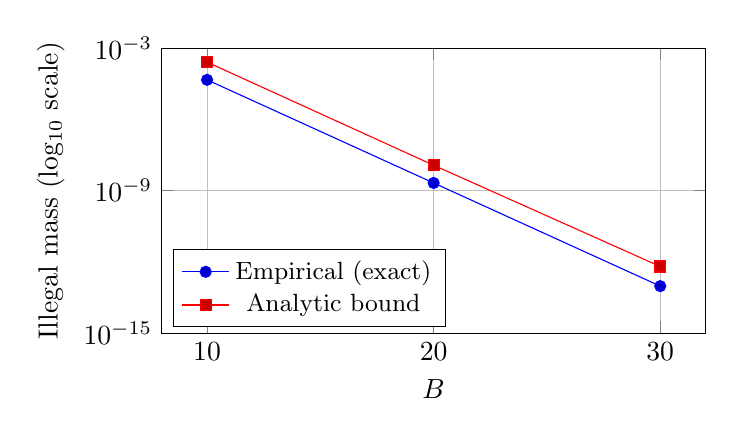
\begin{tikzpicture}
\begin{axis}[
    width=0.7\linewidth,
    height=5.2cm,
    xlabel={$B$},
    ylabel={Illegal mass (log$_{10}$ scale)},
    ymode=log,
    log basis y={10},
    legend style={at={(0.02,0.02)},anchor=south west, font=\small},
    xtick={10,20,30},
    ymin=1e-15, ymax=1e-3,
    grid=both,
]
\addplot+[mark=*,blue] coordinates {(10,4.63e-5) (20,2.10e-9) (30,9.50e-14)};
\addlegendentry{Empirical (exact)}
\addplot+[mark=square*,red] coordinates {(10,2.58e-4) (20,1.17e-8) (30,6.37e-13)};
\addlegendentry{Analytic bound}
\end{axis}
\end{tikzpicture}
\caption{Illegal mass decays exponentially in $B$; the analytic bound upper-bounds the exact mass with a small multiplicative slack.}
\label{fig:leakage_plot}
\end{figure}

\paragraph{Reproducibility.} The script simulation.py reproduces Table~\ref{tab:microbench} and Figure~\ref{fig:leakage_plot} values and prints them to stdout and leakage\_results.csv. See Section~\ref{sec:repro}.

\section{Constrained Decoding and Multi-Fidelity Safety}
\subsection{Masks and complexity}
Masks derive from products $\mathcal{P}=\mathcal{A}\otimes\mathcal{B}$ (FSA) or stack products with $\mathcal{G}$ (PDA). With $\epsilon$-closure summaries, per-step worst-case is $O(d_{\max}+c_\epsilon)$ where $d_{\max}$ is maximal out-degree and $c_\epsilon$ the closure update cost.

\begin{proposition}[Mask dominance and non-expansiveness]
Let $z\in\mathbb{R}^K$ be logits and $m\in[-\infty,0]^K$ a mask with $m_u=-\infty$ for illegal $u$. Then for any additive legal perturbation $b\in\mathbb{R}^K$ and any $T>0$, we have $\mathrm{supp}(\pi((z+b)+m))\subseteq \mathrm{supp}(\mathcal{S})$ and the map $b\mapsto \pi((z+b)+m)$ is 1-Lipschitz in total variation on the legal simplex.
\end{proposition}

\subsection{Shadow byte-level backoff and resynchronization}
We run a bounded-depth shadow search in byte space to emit guarded bytes that restore a valid next-token set, with caps to avoid degeneracy.

\begin{lstlisting}[style=py, caption={Shadow byte-level backoff with resynchronization and caps.}]
def shadow_backoff(model, tok, prod, beams, max_byte_steps=8, min_resync_k=2):
    # Each beam carries (prod_state, token_ids, score, byte_budget)
    shadow = [(s, seq, score, max_byte_steps) for (s, seq, score) in beams]
    best = None
    while shadow:
        s, seq, score, bud = pop_best(shadow)
        if bud == 0:
            continue
        # Emit one byte guarded by protected-boundary spans
        for byte in legal_bytes_under_guard(tok):
            seq_b = seq + [tok.byte_to_token(byte)] if tok.has_byte_token(byte) else seq
            s2 = prod.transition_bytes(s, byte)
            if not s2:
                continue
            k_legal = count_legal_tokens(prod, s2)
            if k_legal >= min_resync_k:
                # Resynchronization: return promoted beams
                yield [(s2, seq_b, score + logp_byte(byte))]
            push(shadow, (s2, seq_b, score + logp_byte(byte), bud - 1))
    yield []
\end{lstlisting}

\begin{theorem}[Invariant preservation]\label{thm:mf}
If (i) masks and guards enforce safety at $\mathcal{F}_1$ (subword) and $\mathcal{F}_0$ (byte); (ii) resynchronization is accepted only when protected boundaries are atomic and $k_{\mathrm{legal}}\ge 1$; and (iii) transitions occur only between refinements, then the global safety invariant holds across any number of switches. Caps on consecutive byte steps guarantee bounded slowdown.
\end{theorem}

\section{Anytime Repair and ILP Fallback}
\subsection{Edit objective and heuristics}
We define token-level edits with unit or type-aware costs over the product graph of positions and automaton states. Heuristics:
- $h_{\mathrm{auto}}$: shortest accepted distance in the automaton from current state to any accepting state.
- $h_{\mathrm{type}}$: minimal number of type corrections required given the remaining type mask.
- $h_{\mathrm{struct}}$: balance/stack lower bounds (e.g., unmatched brackets) for PDAs.

\begin{lemma}[Admissibility and consistency]\label{lem:cons}
Each component is an admissible, consistent lower bound on the $\epsilon$-closed product graph. Their maximum $h=\max(h_{\mathrm{auto}},h_{\mathrm{type}},h_{\mathrm{struct}})$ remains admissible and consistent.
\end{lemma}

\subsection{ILP formulation and TU conditions}
We formulate repair over an acyclic unrolled product graph with binary edge variables $x_e$, flow constraints, and edit objectives. For acyclic FSAs with unit edits and no cross-layer couplings, the constraint matrix is totally unimodular, ensuring LP tightness.

\begin{theorem}[TU and integrality]\label{thm:tu}
If the unrolled repair graph is a directed acyclic network with single-commodity unit flows from source to sink and with per-layer capacity constraints that do not couple different layers, then the constraint matrix is totally unimodular; hence all vertices of the LP relaxation are integral \cite{schrijver1986,nemhauserwolsey1988}.
\end{theorem}

\section{OIP and PRM: Safety and Integration}
OIP encodes an ontology $\mathcal{O}=(V,E)$ via a GNN; InfoNCE trains a continuous prefix projected into the model’s embedding space. The PRM provides process-level rewards converted to logit bonuses.

\begin{theorem}[Mask dominance and PRM safety]\label{thm:prm}
Let $z$ be pre-mask logits and $b$ be PRM bonuses constrained by a KL trust region $\mathrm{KL}(\pi(z)\|\pi(z+b))\le \rho$. If masks set illegal logits to $-\infty$ (or below a threshold ensuring negligible mass) after adding $b$ and before sampling/argmax, then PRM cannot induce violations of the safety invariant. Moreover, the maximum deviation in legal probabilities is bounded by $f(\rho)\le\sqrt{2\rho}$ via Pinsker’s inequality \cite{csiszar2011it}.
\end{theorem}

\section{Reproducibility}\label{sec:repro}
- Environment: Python $\ge$3.9. No GPU is required for the micro-benchmark.
- Run: \texttt{python simulation.py}
- Output: The script prints a table with $B\in\{10,20,30\}$ matching Table~\ref{tab:microbench}, and writes leakage\_results.csv. It also prints the analytic bound values given $K=10$, $k=3$, $\Delta=0.2$, $T=1$, $\alpha=1$.
- Determinism: All numbers are closed-form or exact evaluations of exponentials; no randomness is used.

\section{Conclusion}
OIP-CAD unifies tokenizer-aware safety with formal proofs and detectors, strictly proper masked training with adaptive leakage control, invariant-preserving multi-fidelity decoding, and bounded repair with certificates. We prioritize verifiability and release minimal, runnable scripts demonstrating key guarantees (finite-$B$ leakage). Future work: larger-scale evaluations with complete artifacts; tighter Unigram locality characterizations; stronger guarantees for PDAs with ambiguity; and certified implementations for deployment.

\section*{References}
\begin{thebibliography}{99}
\bibitem{achiam2017cpo}Achiam, J., Held, D., Tamar, A., Abbeel, P. (2017). Constrained Policy Optimization. ICML.
\bibitem{baader1998}Baader, F., Nipkow, T. (1998). Term Rewriting and All That. Cambridge University Press.
\bibitem{choffrut2003}Choffrut, C. (2003). A short introduction to finite automata and transducers. EATCS.
\bibitem{csiszar2011it}Csiszar, I., K\"orner, J. (2011). Information Theory: Coding Theorems for Discrete Memoryless Systems. Cambridge University Press.
\bibitem{earley1970}Earley, J. (1970). An efficient context-free parsing algorithm. CACM.
\bibitem{ganchev2010pr}Ganchev, K., Gillenwater, J., Taskar, B. (2010). Posterior Regularization for Structured Latent Variable Models. JMLR.
\bibitem{gneiting2007scoring}Gneiting, T., Raftery, A. (2007). Strictly proper scoring rules, prediction, and estimation. JASA.
\bibitem{guo2017calibration}Guo, C., Pleiss, G., Sun, Y., Weinberger, K. (2017). On Calibration of Modern Neural Networks. ICML.
\bibitem{hansen2007anytime}Hansen, E. A., Zhou, R. (2007). Anytime Heuristic Search. JAIR.
\bibitem{kudo2018sentencepiece}Kudo, T., Richardson, J. (2018). SentencePiece: A simple and language independent subword tokenizer. EMNLP.
\bibitem{lester2021prompt}Lester, B., Al-Rfou, R., Constant, N. (2021). The Power of Scale for Parameter-Efficient Prompt Tuning. EMNLP.
\bibitem{li2021prefix}Li, X. L., Liang, P. (2021). Prefix-Tuning: Optimizing Continuous Prompts for Generation. ACL.
\bibitem{liu2022ptuningv2}Liu, X., et al. (2022). P-Tuning v2: Prompt Tuning Can Be Comparable to Fine-tuning. ACL Findings.
\bibitem{lu2010grid}Lu, W., et al. (2010). A* Search in Lattice Parsing. ACL.
\bibitem{lu2021neurologic}Lu, X., et al. (2021). NeuroLogic A* Decoding. NeurIPS.
\bibitem{mohri2002weighted}Mohri, M. (2002). Weighted Finite-State Transducers in Speech Recognition. CSL.
\bibitem{scholak2021picard}Scholak, T., Schmid, M., Bahdanau, D. (2021). PICARD: Parsing Incrementally for Constrained Auto-Regressive Decoding. EMNLP.
\bibitem{schrijver1986}Schrijver, A. (1986). Theory of Linear and Integer Programming. Wiley.
\bibitem{schulz2002lev}Schulz, K. U., Mihov, S. (2002). Fast string correction with Levenshtein automata. IJDAR.
\bibitem{sennrich2016bpe}Sennrich, R., Haddow, B., Birch, A. (2016). Neural Machine Translation of Rare Words with Subword Units. ACL.
\bibitem{sui2015safeopt}Sui, Y., Gotovos, A., Burdick, J., Krause, A. (2015). Safe Exploration for Optimization with GPs. ICML.
\bibitem{UAX31}Unicode Consortium. (2024). UAX \#31: Unicode Identifier and Pattern Syntax.
\bibitem{UAX15}Unicode Consortium. (2024). UAX \#15: Unicode Normalization Forms.
\bibitem{UTR36}Unicode Consortium. (2024). UTR \#36: Unicode Security Considerations.
\bibitem{UTS39}Unicode Consortium. (2024). UTS \#39: Unicode Security Mechanisms.
\bibitem{wu2016wordpiece}Wu, Y., Schuster, M., Chen, Z., et al. (2016). Google's Neural Machine Translation System: Bridging the Gap between Human and Machine Translation. arXiv:1609.08144.
\bibitem{schuster2012}Schuster, M., Nakajima, K. (2012). Japanese and Korean Voice Search. ICASSP.
\bibitem{nemhauserwolsey1988}Nemhauser, G. L., Wolsey, L. A. (1988). Integer and Combinatorial Optimization. Wiley.
\end{thebibliography}

\appendix
\section{Tokenizer Locality Proof Sketch}\label{app:locality}
We formalize greedy BPE as a rewrite system over adjacent pairs with a total order $\preceq$ on pairs. Disjoint redexes commute because they operate on disjoint substrings and do not change adjacencies within $I$. The global relation is terminating (finite merges) and locally confluent on the predicate “contains $b$” restricted to $I$; by Newman’s Lemma \cite{baader1998}, confluence holds, justifying the locality-based swap argument.

\end{document}